\documentclass{tufte-book}
\title{电路}
\author{肖书奇}
\publisher{2022年}
\usepackage{ifxetex}% For compatibility with xelatex engine
    \ifxetex
    \newcommand{\textls}[2][5]{%
        \begingroup\addfontfeatures{LetterSpace=#1}#2\endgroup
    }
    \renewcommand{\allcapsspacing}[1]{\textls[15]{#1}}
    \renewcommand{\smallcapsspacing}[1]{\textls[10]{#1}}
    \renewcommand{\allcaps}[1]{\textls[15]{\MakeTextUppercase{#1}}}
    \renewcommand{\smallcaps}[1]{\smallcapsspacing{\scshape\MakeTextLowercase{#1}}}
    \renewcommand{\textsc}[1]{\smallcapsspacing{\textsmallcaps{#1}}}
    \usepackage[osf,sc]{mathpazo} % tufte style font
    \usepackage[scaled=0.90]{helvet} % tufte style font
    \usepackage[scaled=0.85]{beramono} % tufte style font
    \fi
\usepackage{ctex} % 支持中文
\usepackage{xeCJK}% 支持中文
    \xeCJKsetup{PunctStyle=kaiming}  % 设置中文标点符号,开明式
    % \xeCJKsetup{PunctStyle=quanjiao} % 设置中文标点符号,全角式
    % \setCJKmainfont{仓耳今楷05-6763}      % 设置正文罗马族的 CJK 字体,影响 \rmfamily 和 \textrm 的字体。
    % \setCJKmainfont{STZhongsong}      % 设置正文罗马族的 CJK 字体,影响 \rmfamily 和 \textrm 的字体。
    % \setCJKsansfont{STZhongsong}  % 设置正文无衬线族的 CJK 字体,影响 \sffamily 和 \textsf 的字体。
    % \setCJKmonofont{SimHei}          % 设置正文等宽族的 CJK 字体,影响 \ttfamily 和 \texttt 的字体。
\usepackage{amsmath} % For AMS math support
\usepackage{amssymb} % For AMS math support
\usepackage{amsfonts} % For AMS math support
\usepackage{booktabs} % For nicely typeset tabular material
\usepackage{makecell} % For multiple lines in one cell in table environment
\usepackage{diagbox}
\usepackage{adjustbox}
\usepackage{graphicx} % For graphics / images
    \setkeys{Gin}{width=\linewidth,totalheight=\textheight,keepaspectratio} % Set default scale globally
    \graphicspath{{../graphics/}} % Set paths to search for images
\usepackage{makeidx} % For index
    \makeindex
\usepackage{romannum} % For Roman numbers
\usepackage[dvipsnames]{xcolor} % For various colors
    % \pagecolor{black}
    % \color{white}
\hypersetup{colorlinks} % For colored hyperlinks             
\setcitationfont{\normalfont\footnotesize\color{gray}}
\begin{document}
\frontmatter% Front matter
\maketitle
\tableofcontents% TOC

\chapter{大局观}
\adjustbox{trim={.15\width} {.35\height} {0.15\width} {.1\height},clip}
{
    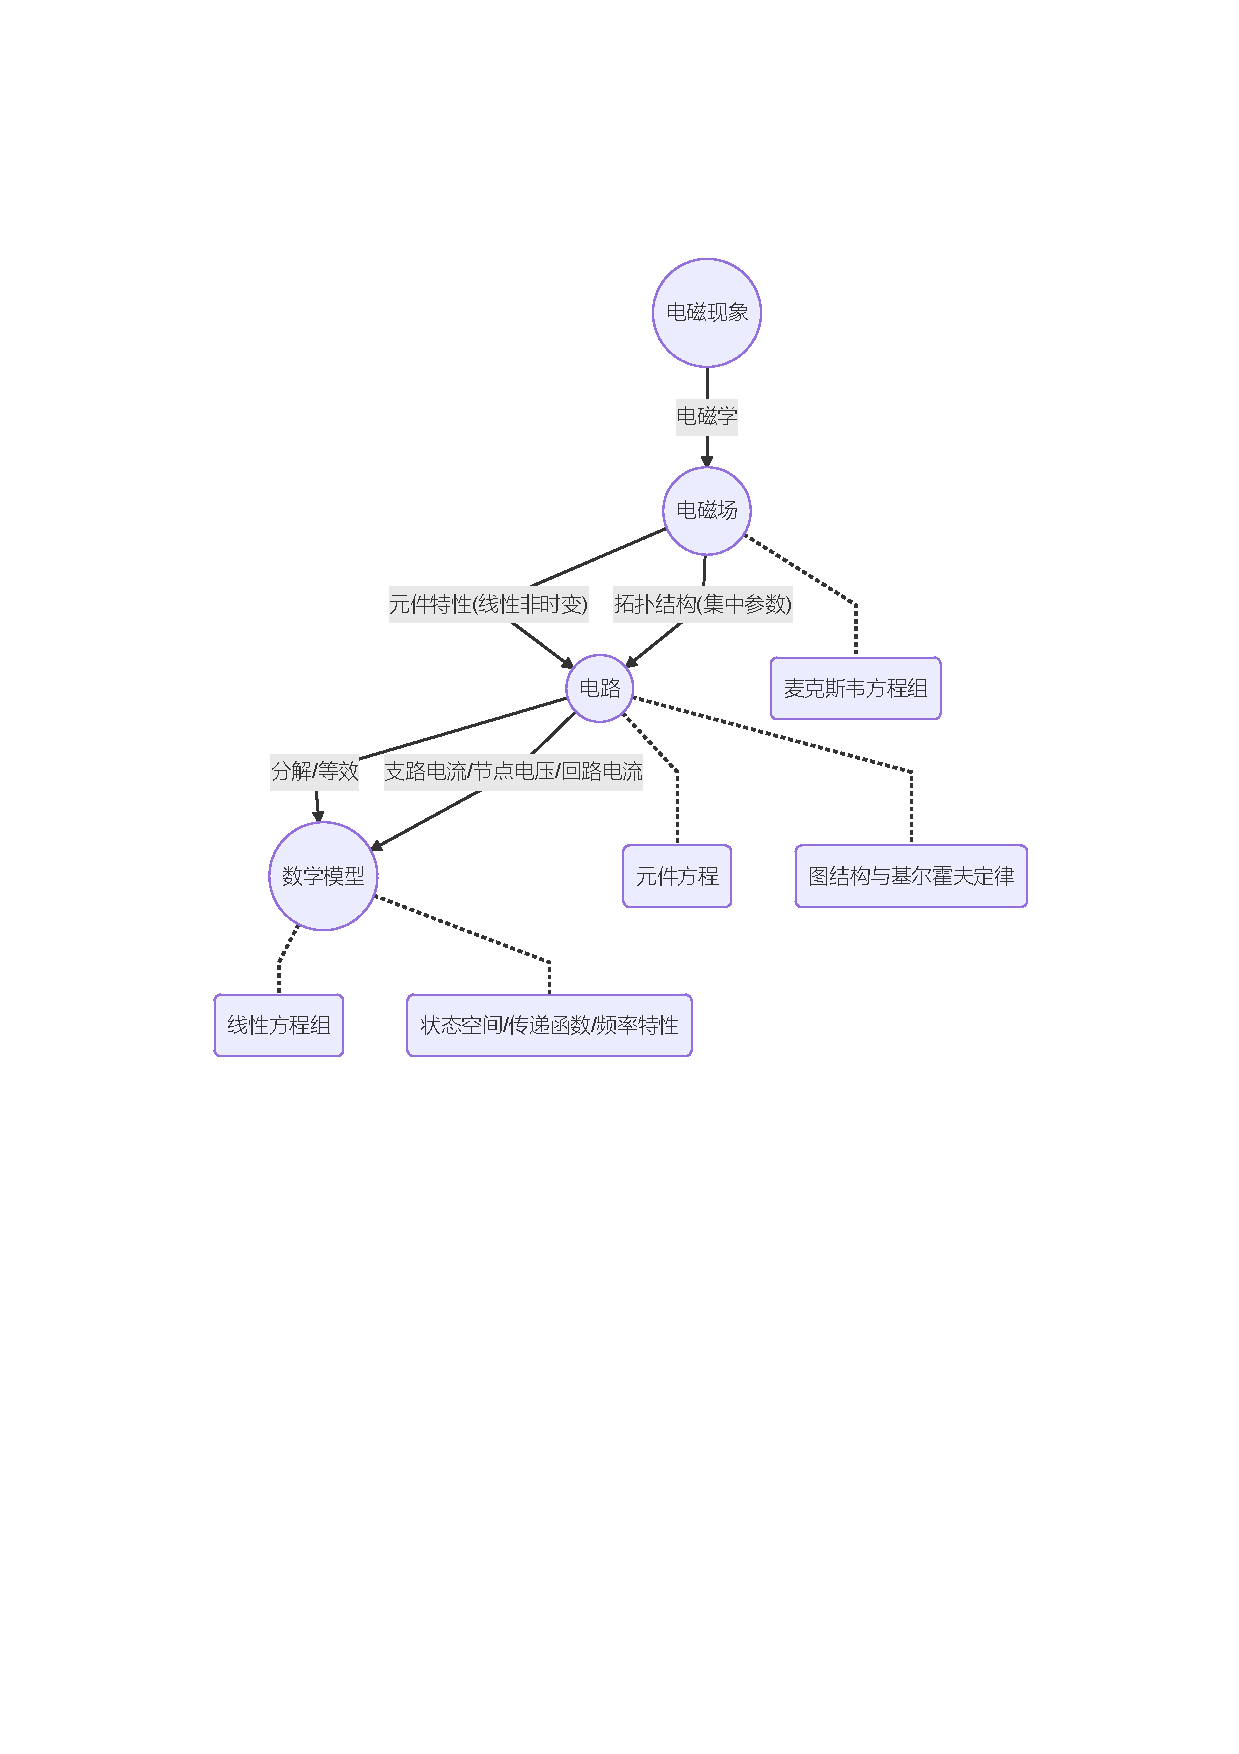
\includegraphics[width=\textwidth]{大局观.pdf}
}
\chapter{线性电阻电路的一般分析方法}
\adjustbox{trim={.15\width} {.2\height} {0.15\width} {.1\height},clip}
{
    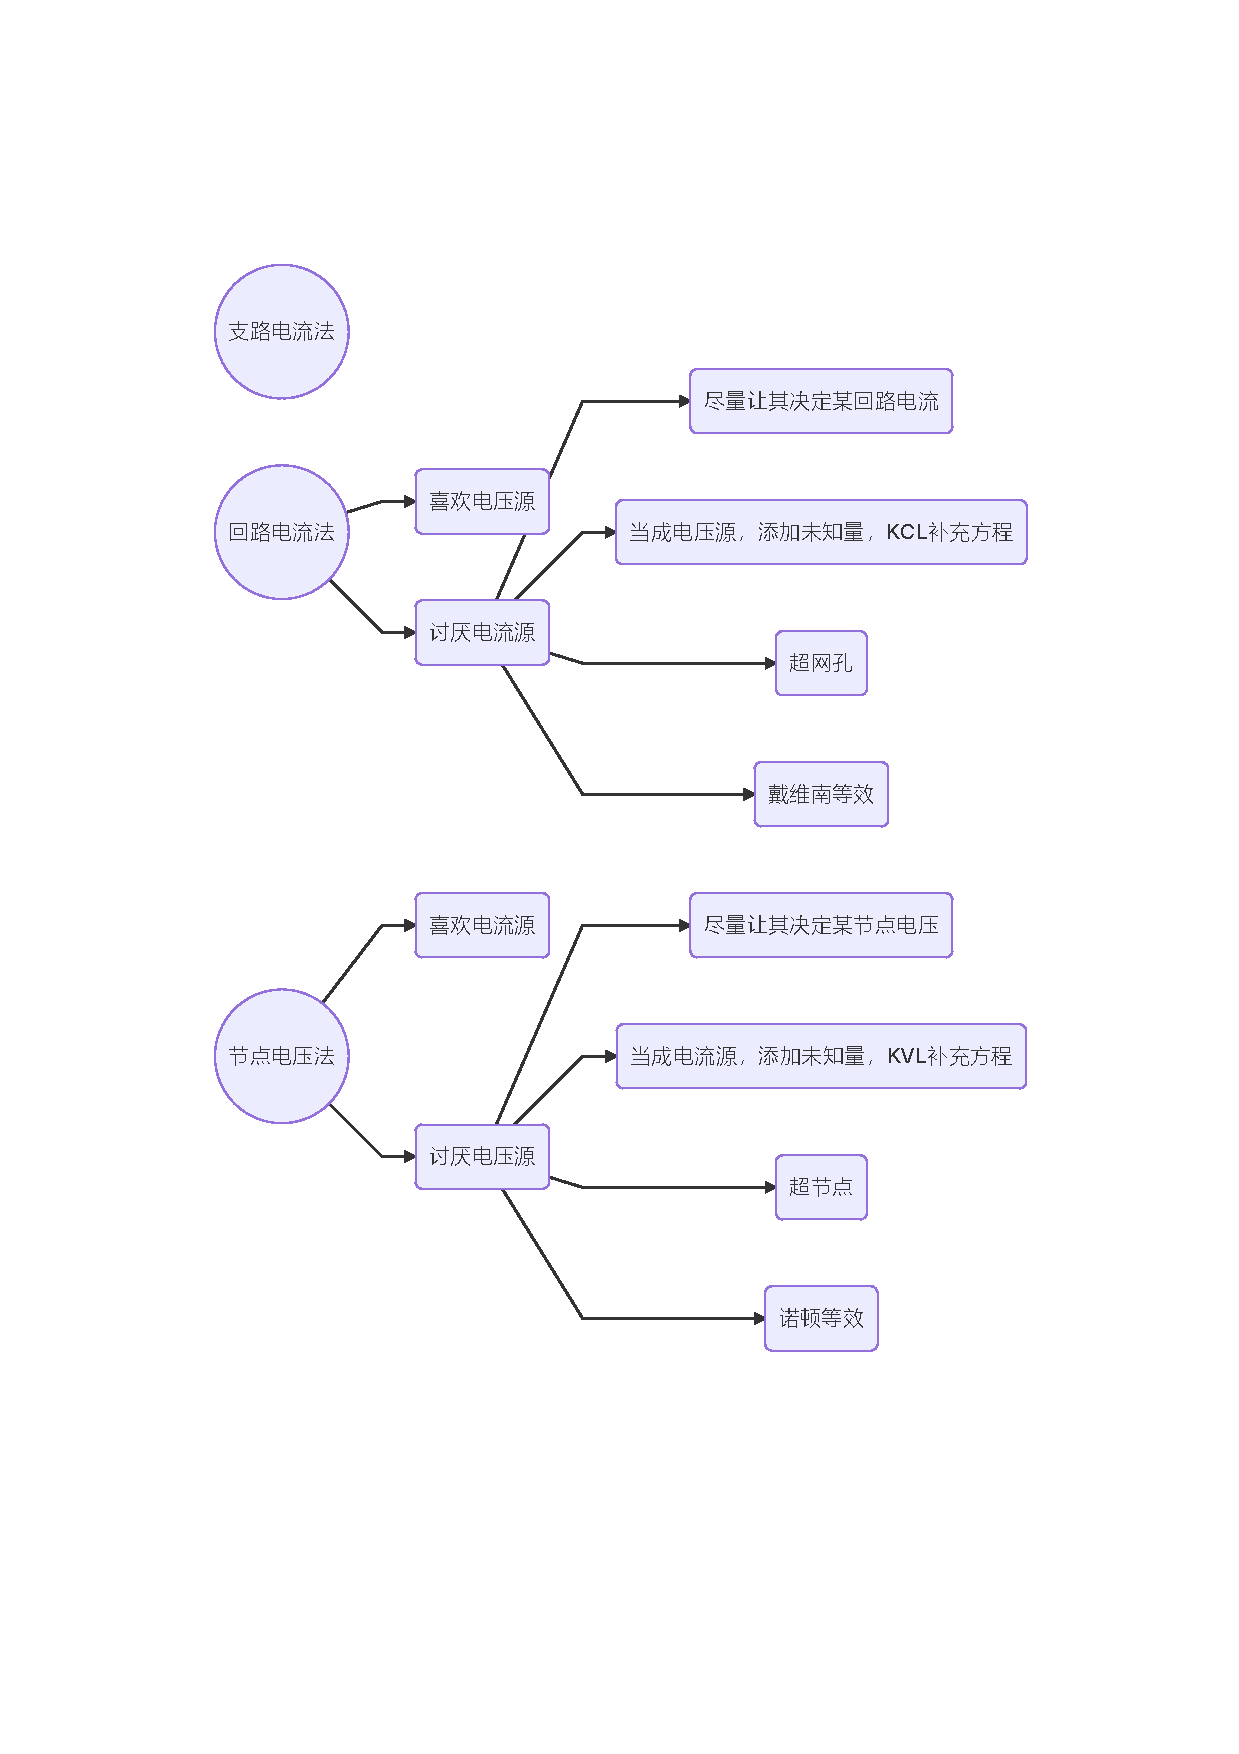
\includegraphics[width=\textwidth]{线性电阻电路的一般分析方法.pdf}
}
闷头写出某个回路/节点的自导/自阻可能会出的问题
\begin{itemize}
    \item 该回路电流/节点电压已经被决定,不能正常列方程;
    \item 与理想电压源并联的电阻;与理想电流源串联的电阻。
\end{itemize}
思考流程:
\begin{enumerate}
    \item 观察独立节点数目、独立回路数目;
    \item 观察电压源数目、电流源数目;
    \item 综合1,2点决定节点电压或回路电流法;
    \item 观察可否等效;
    \item 选择处理讨厌情况的方法,心中默念其易错点;
    \item 标记
    \item 开始列方程
\end{enumerate}
\backmatter

% % \bibliography{}
% % \bibliographystyle{plainnat}
\printindex
\end{document}
